\documentclass[12pt]{article}
\usepackage{sbc-template}
\usepackage{graphicx,url}
\usepackage{float}
\usepackage[brazil]{babel}   
\usepackage[utf8]{inputenc}  
\usepackage{url}
\bibliographystyle{ieeetr}

\usepackage{inconsolata}

\usepackage{color}

\definecolor{pblue}{rgb}{0.13,0.13,1}
\definecolor{pgreen}{rgb}{0,0.5,0}
\definecolor{pred}{rgb}{0.9,0,0}
\definecolor{pgrey}{rgb}{0.46,0.45,0.48}

\usepackage{listings}
\lstset{language=Java,
	showspaces=false,
	showtabs=false,
	breaklines=true,
	showstringspaces=false,
	breakatwhitespace=true,
	commentstyle=\color{pgreen},
	keywordstyle=\color{pblue},
	stringstyle=\color{pred},
	basicstyle=\ttfamily
}
     

\sloppy
	\title{ Simulação de Pool de Impressão Dístribuida Utilizando Socket \\ Exercício Computacional II - Sistemas Distribuídos}

\author{Rafael Gonçalves de Oliveira Viana\inst{1}  }


\address{Sistemas de Informação -- Universidade Federal do Mato Grosso do Sul
	(UFMS)\\
  	Caixa Postal 79400-000 -- Coxim -- MS -- Brazil
  \email{rafael.viana@aluno.ufms.br }
  \\\vspace*{10pt} \normalsize  \today{}
}

\begin{document} 

\maketitle

     
\begin{resumo} 	
  Este  documento relata os pontos fortes no desenvolvimento de uma Pool de Thread na linguaguem Java versão 8.
\end{resumo}

\section{Introdução}
 De acordo com \cite{entf}, em um ambiente de trabalho, onde desejasse imprimir documentos enviados, a um curto período de tempo, é necessario a utilização de uma pool de impressão.
 
 Uma pool de impressão permite que várias impressoras físicas possam ser controladas por uma única impressora lógica,  sempre que um trabalho for enviado para a impressora lógica, esta consultará o estado das impressoras físicas para verificar qual equipamento está livre no momento e enviará o trabalho para ela .
Um exemplo de pool de impressão é demostrada na figura \ref{fig:screenshot001}.
\begin{figure}[H]
 	\centering
 	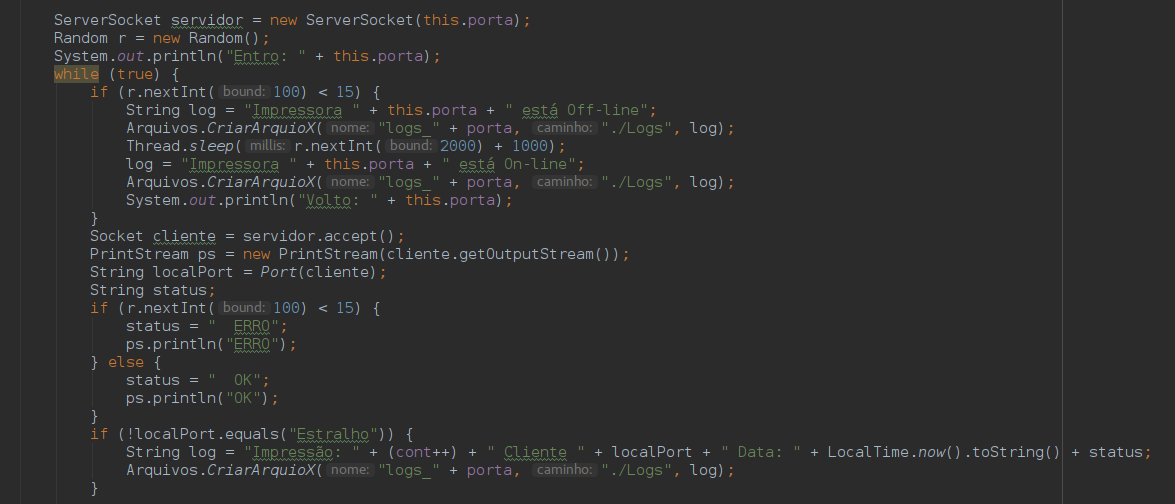
\includegraphics[width=0.7\linewidth]{imagens/screenshot001}
 	\caption{Proposta do exercício computacional.}
 	\label{fig:screenshot001}
 \end{figure}
 
\section{Fundamentação Téorica} 
	Nesta sessão serão tradatas, as tecnologias que foram utilizadas neste documento.
 
\subsection{Socket}
 Segundo \cite{socket}.\cite{conc}.
 Os sockets são compostos por um conjunto de primitivas do sistema operacional e foram originalmente desenvolvidos para o BSD Unix. Podem ser utilizados nos mais variados sistemas operacionais com recursos de comunicação em rede, sendo suportados pela maioria das linguagens de programação. Sockets são suportados em Java desde o JDK 1.0, para sua utilização devemos fazer uso das classes contidas no pacote java.net. Um exemplo interessante da programação de sockets em Java são os drivers JDBC do tipo 4, que usam sockets para comunicar-se diretamente com a API de rede do banco de dados. O fluxo de troca de dados de um socket pode ser observada na figura \ref{fluxoSocket}.
\begin{figure}[H]
	\centering
	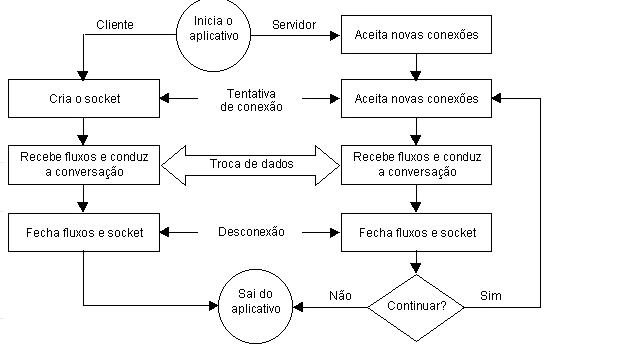
\includegraphics[scale=1]{imagens/fluxoSocket.JPG}
    \caption{Fluxo de troca de dados com sockets.}
	\label{fluxoSocket}
\end{figure}

 \subsection{Problema de Concorrência}
Essa ideia é chamada de região crítica. É um pedaço de código que definimos como crítico e que não pode ser executado por duas threads ao mesmo tempo. Apenas uma thread por vez consegue entrar em alguma região crítica.

\section{Desenvolvimento}
Para resolver o trabalho proposto, foi desenvolvido uma aplicação java que simula, uma pool de impressões que as ordena e envia para uma impressora.
	Foram criadas 3 classes Javas sendo elas: Cliente , Pool de Impressão e Impressora.
	 As mesmas serão comentandas nas póximas sessões.
\subsection{Cliente}
	Essa classe  se conecta a classe servidor, repassando informações via Socket, em uma via de mão dupla.
	Os dados serão aceitos na memória e posteriormente serão alocados no pelo escalonardo da pool de impressão, em alguma impressora disponível, onde mais tarde será notificado com o resultado da processamento da impressão.
	
	O código responsável pela chamda de impressão no cliente e simples, podemos observar o método na figura  \ref{fig:screenshot005}.
\begin{figure}[H]
	\centering
	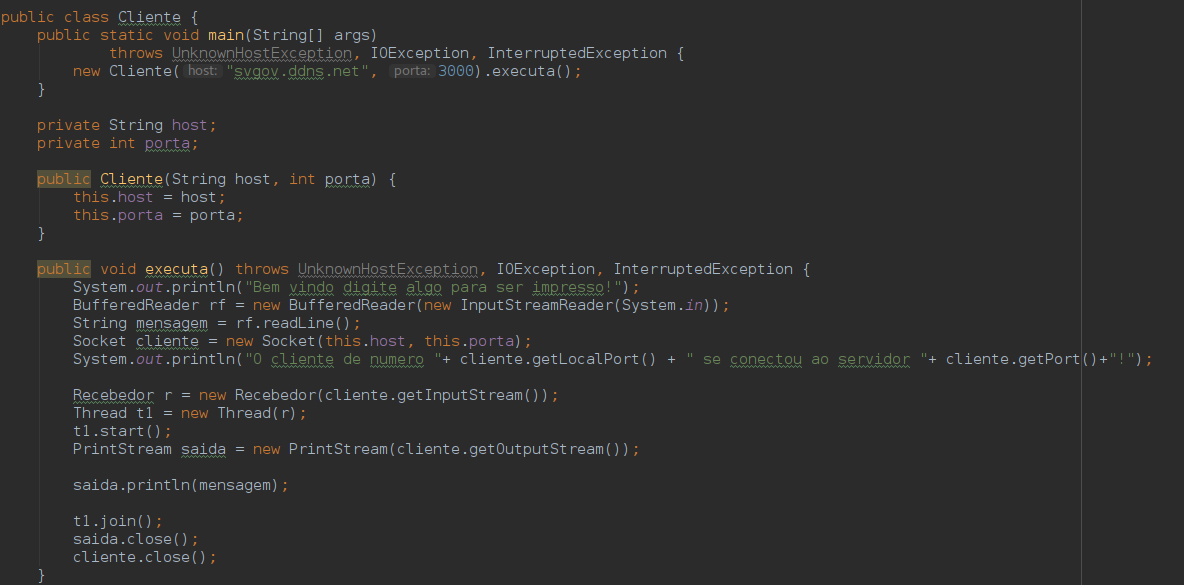
\includegraphics[width=1\linewidth]{imagens/screenshot005}
	\caption{Código cliente, pool de impressão.}
	\label{fig:screenshot005}
\end{figure}



\subsection{Pool de Impressão - Servidor}\label{pool}
  Classe responsável pela comunicação dos Sockets (Cliente/Impressora), ela contém o escalonador  de impressão, que  é responsável por designar os serviços na pool de impressão.
  
	  O código do servidor é responsável por 3 threads sendo elas:
	  \begin{enumerate}
	  	\item Aceitar conexões via Socket e adicionar documento para impressão.
	  	\item Procurar impressoras disponíveis (escalonador de impressão)
	  	\item Enviar documento para impressoras e receber resposta de confirmação das mesmas.
	  \end{enumerate}
	
	A figura \ref{fig:screenshot006} demostra a função que inicializa as variáveis proposta no exercício computacional, além de iniciar as Threads do servidor. 

\begin{figure}[H]
	\centering
	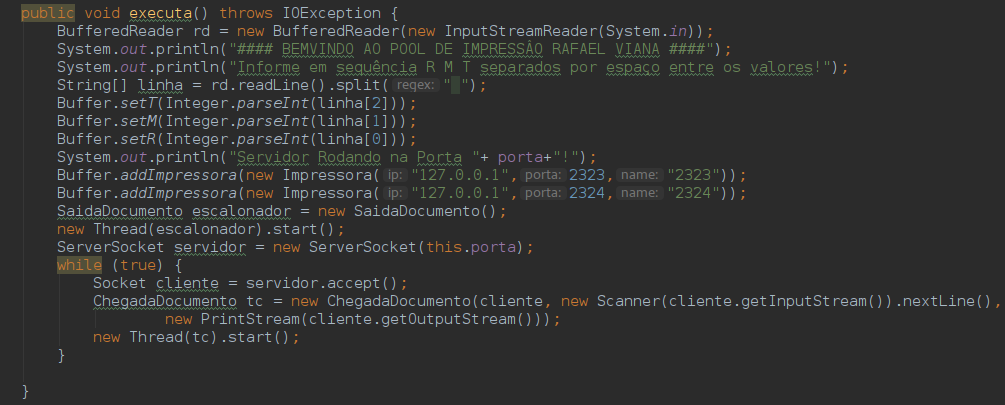
\includegraphics[width=0.7\linewidth]{imagens/screenshot006}
	\caption{}
	\label{fig:screenshot006}
\end{figure}
O código completo, incluindo todas as classes como na figura \ref{fig:screenshot008}, estão disponíveis no link https://github.com/rafaelgov95/SD/tree/master/PTJI/Projeto-PTJ
\begin{figure}[H]
	\centering
	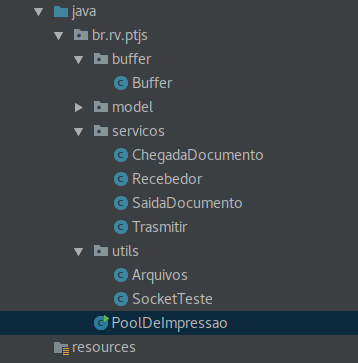
\includegraphics[width=0.4\linewidth]{imagens/screenshot008}
	\caption{Classes do Servidor de pool de Impressão}
	\label{fig:screenshot008}
\end{figure}


\subsection{Impressoras}
	Classe responsável pela impressão dos documentos contidos  no buffer da Pool de Impressão \ref{pool}.
	
	Ela trabalha junto ao escalonador do servidor, que é responsável por notificada as impressoras cadastradas, que novas impressões devem ser executadas.
	
	A figura \ref{fig:screenshot002}, apresenta o método que realiza a criação das Threads.
	Elas executam em modo servidor aguardando o escalonador alocar alguma tarefa.
\begin{figure}[H]
	\centering
	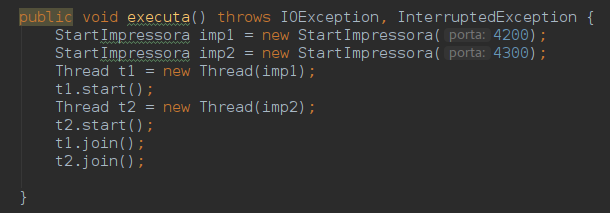
\includegraphics[width=0.7\linewidth]{imagens/screenshot002}
	\caption{Criação de 2 impressoras pelo método StartImpressora.}
	\label{fig:screenshot002}
\end{figure}

Após acriação, as Threads que representam as impressoras, ficam aguardando no while(), pelo método servidor.accept como na figura  \ref{fig:screenshot004}.


\begin{figure}[H]
	\centering
	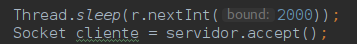
\includegraphics[width=0.7\linewidth]{imagens/screenshot004}
	\caption{}
	\label{fig:screenshot004}
\end{figure}
O código do laço completo e demostrado na figura \ref{fig:screenshot003}.

\begin{figure}[H]
	\centering
	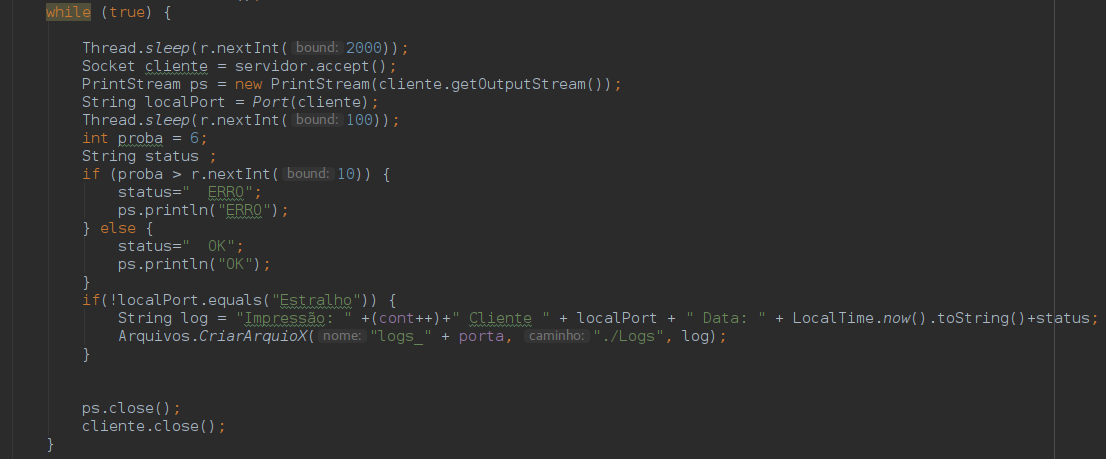
\includegraphics[width=0.7\linewidth]{imagens/screenshot003}
	\caption{}
	\label{fig:screenshot003}
\end{figure}
\section{Testes e Resultados }
 Nesta sessão será demostrado os relatórios após  a conexão de 4 clientes, com o servidor e posteriormente a distribuição dos documentos entre as impressoras disponíveis. 
 Após o processamento uma resposta de impressão é encaminhada para os clientes.
 O relatório do escalonador, após a execução dos
 4 clientes é demostrado na figura \ref{fig:screenshot009}.
 \begin{figure}[H]
 	\centering
 	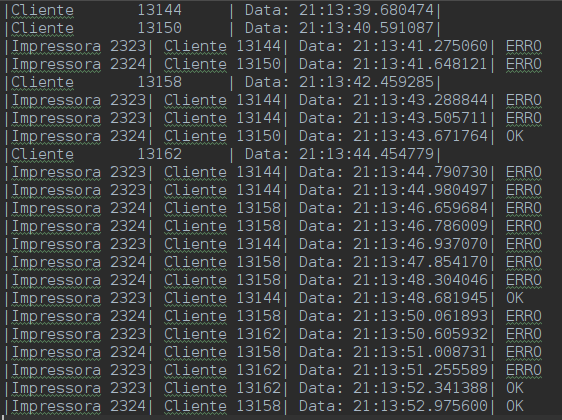
\includegraphics[width=0.7\linewidth]{imagens/screenshot014}
 	\caption{Relatório de impressões, registrado pelo escalonador presente no servidor.}
 	\label{fig:screenshot009}
 \end{figure}

 
 O relatório da impressora 2323, pode ser observado na figura \ref{fig:screenshot010}.

 \begin{figure}[H]
 	\centering
 	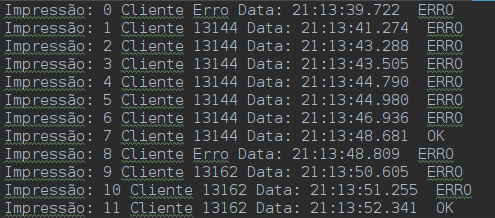
\includegraphics[width=0.7\linewidth]{imagens/screenshot013}
 	\caption{Relatório da impressora 2323, após execução dos 4 clientes.}
 	\label{fig:screenshot010}
 \end{figure}
 
  O relatório da impressora 2324, pode ser observado na figura \ref{fig:screenshot012}.
  \begin{figure}[H]
  	\centering
  	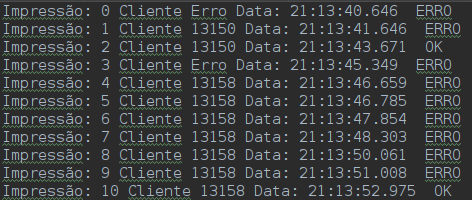
\includegraphics[width=0.7\linewidth]{imagens/screenshot012}
  	\caption{Relatório da impressora 2324, após execução dos 4 clientes.}
  	\label{fig:screenshot012}
  \end{figure}
  
  O cliente após  o envio do documento, aguarda a impressão do mesmo, enquanto isso recebe notificações  a respeito de sua impressão em tempo real, podemos ver  na figura  \ref{fig:screenshot015}, o resultado final de notificações do cliente.
  
  \begin{figure}[H]
  	\centering
  	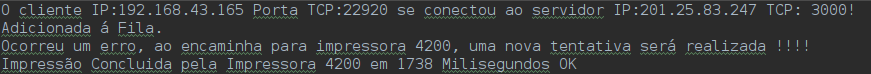
\includegraphics[width=0.7\linewidth]{imagens/screenshot015}
  	\caption{Notificações em tempo real da impressão para o Cliente.}
  	\label{fig:screenshot015}
  \end{figure}
  
\section{Conclusão}
Neste relatório foi apresentado  o desenvolvimento de uma pool de impressão, assim como a problematica da região crítica de mémoria compatilhada entre Threads, e a sua solução utilizando  o \textit{synchronized}.
Para realizar a comunicação entre as Threads foram utilizadas conexões Sockets.


\bibliography{bibli}

\end{document}


